\documentclass[platex,dvipdfmx,a4paper,twocolumn,base=10pt,jbase=10pt,ja=standard]{bxjsarticle}
% \documentclass[uplatex,dvipdfmx,a4paper,twocolumn,base=11pt,jbase=11pt,ja=standard]{bxjsarticle}
% https://github.com/yk-lab/ipsj_national_convention_template

\usepackage{ipsj}

\usepackage[dvipdfmx]{graphicx}
\usepackage{amsmath,amsfonts}
\usepackage{bm}

% \def\baselinestretch{1.0}
\def\baselinestretch{0.9}  % 0.86

\title{\Large\bf 電子教材の閲覧データとコンテンツ内容を用いた\\学習者のスコア予測}{\bf Predicting learner scores using browsing data and content of electronic learning materials}
\author{兵庫県立大学 社会情報科学部}{小岸 沙也加}{Sayaka Kogishi, University of Hyogo}
\author{九州大学 システム情報科学研究院}{峰松 翼}{Tsubasa Minematsu, Kyushu University}
\author{九州大学 システム情報科学研究院}{島田 敦士}{Atsushi Shimada, Kyushu University}
\author{兵庫県立大学 情報科学研究科}{川嶋 宏彰}{Hiroaki Kawashima, University of Hyogo}

\begin{document}
\maketitle

\section{はじめに}
\label{sec:intro}
    
近年、学校の講義では講義資料の閲覧や課題の提出等で小学生から大学生まで幅広くタブレットやノートPCが使われている.講義資料はPDFとして自分のPCにダウンロードしてオフラインで閲覧するだけではなく,web上に教師が講義資料をアップロードしてwebを経由してオンライン上で操作できる,e-Bookシステムが使用され,閲覧される.オンライン所うで講義資料を閲覧することで,どの学生がいつ,どのコンテンツのどのページでどんな操作をしたかという学生の詳細な閲覧データが取得できる.
そこで本研究ではデジタル教材の配信システムのひとつでのひとつである,BookRollシステムから得た閲覧データを用いて学生の学習行動から各学生に対し教材の理解度推定を行う.学生の学習行動から理解度推定ができれば,小テストや定期テストの前の早い段階で各個人に適したアプローチすることができるようになり,学生の学力向上に繋がると期待できる.

% 本研究では理解度を小テストの点数として,閲覧データだけでなく,実際に講義で用いられたコンテンツ内容を使用し毎週講義後に行われる小テストの点数予測を行う.学生の行動に焦点をあて,点数予測を行っている例は以前にもあるため,コンテンツ内容を含めることでどこまで精度があがるのかという点を本研究のリサーチクエスチョンにあげる.

本研究では理解度を小テストの点数として,毎週講義後に行われる小テストのスコア予測を行う.予測には閲覧データだけではなく,実際に講義で用いられたコンテンツの内容を使用する.学生の閲覧行動のみを用いる場合と,コンテンツ内容を含めた場合とで,予測精度がどのように変化するかを評価する.本研究のRQはコンテンツ内容を含めることでどこまで精度があがるのかである.



\section{関連研究}
\label{sec:Related}

学生の行動から成績予測を行った研究として,
~\cite{Predictionstudentperformance2022}ではBookRollシステムで取得した講義資料の読書行動から毎週の生徒の成績を予測し,講義が終わる前にリスクのある生徒とリスクのない生徒に分類することが可能と発表している.

BookRolシステムから得たデータを使用した研究として,~\cite{BR12020}ではLRPというニューラルネットワークの解釈手法を用いて最終成績の上位,中位,下位の分類を行っている.



\section{BookRollシステム}
\label{sec:BookRoll}

BookRollシステムは,教員がアップロードした講義資料や教材を学生がオンライン上で閲覧できるシステムである.図1にBookRollシステムの操作画面の一例を示す.BookRollシステムでは各ページに対しブックマーク,メモの記入,マーカーをつける,コンテンツ内検索などができる.

\vspace{-10mm}

\begin{figure}[h]
  \centering
  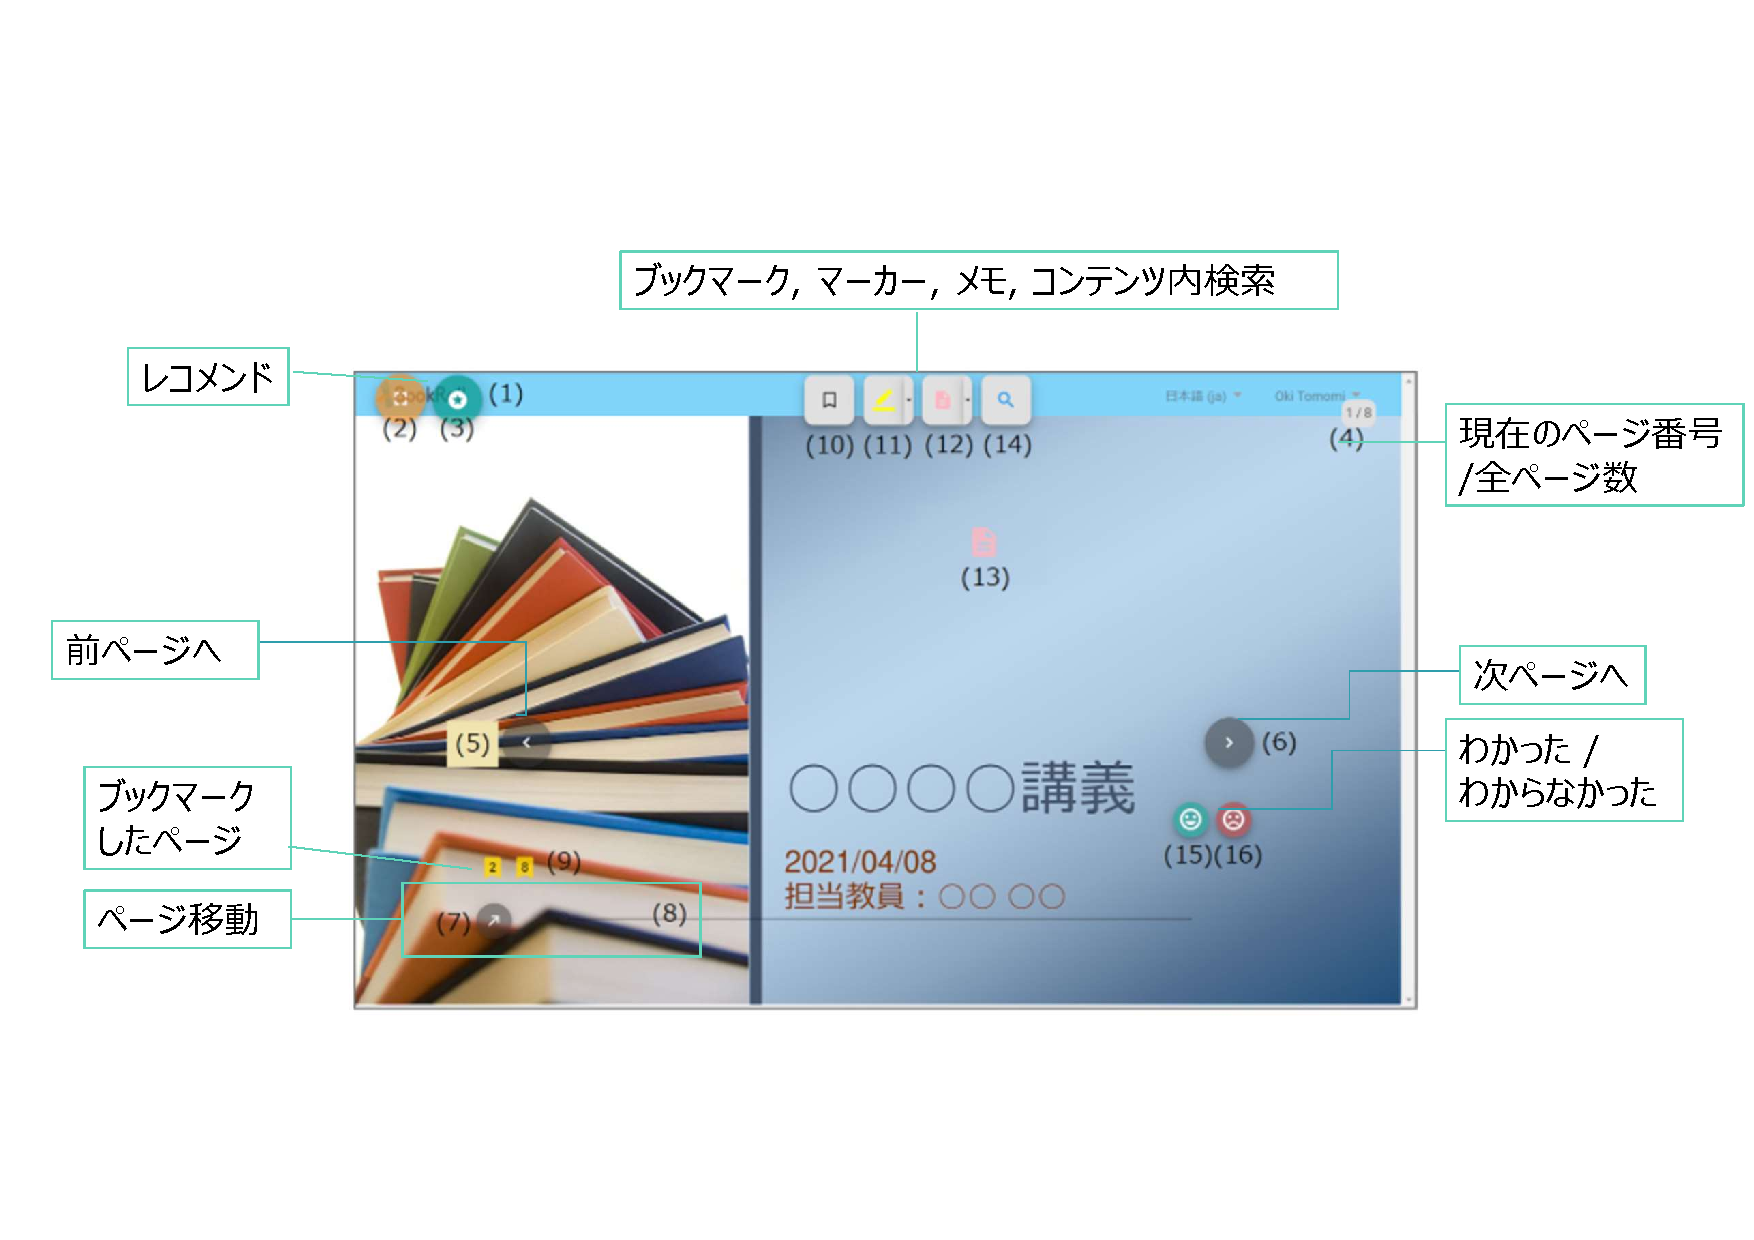
\includegraphics[scale = 0.3]{BookRoll.pdf}
  \vspace{-15mm}
  \caption{BookRollシステム操作画面例}
  \label{fig:BookRollシステム操作画面例}
\end{figure}

% 閲覧データはコンテンツを開く,閉じる,次のページへ進む,一つ前のページへ戻るなどの行動がされたタイミングで操作を行った学生のID,行動をした日時,コンテンツ番号,ページ番号,どのような操作を行ったか等の情報が記録される.記録される主な内容を表1に示す.表1のoperation\_nameにあたる,閲覧データに記録される操作の一部を表2に示す.

閲覧データはコンテンツを開く,閉じる,次のページへ進む,一つ前のページへ戻るなどの行動がされたタイミングで操作を行った学生のID,行動をした日時,コンテンツ番号,ページ番号,どのような操作を行ったか等の情報が記録される.
記録される操作には,ページ移動,マーカー,メモ,ブックマークをつける/消す,コンテンツ内検索を行うなどが含まれる.

% \begin{table}[h]
%   \centering
%   \begin{tabular}{c|l}
%     記録名 & 内容 \\ \hline
%     contents\_id/name & コンテンツID/名 \\ 
%     marker\_position/color & マーカーをつけた場所/色 \\ 
%     memo\_text & メモの内容 \\
%     operation\_date & 操作した日時 \\ 
%     operation\_name & 操作内容 \\ 
%     page\_no & 操作したページ番号 \\ 
%     userid & 学生に割り振られた番号 \\ \hline
%   \end{tabular}
%   \caption{記録される主な内容}
%   \label{tb:記録される主な内容}
% \end{table}

% \begin{table*}[h]
%   \centering
%   \begin{tabular}{c|l}
%     operation\_name & 内容 \\ \hline
%     OPEN & コンテンツを開く \\ 
%     CLOSE & コンテンツを閉じる \\ 
%     NEXT & 次のページへ移動 \\
%     PREV & ひとつ前のページへ移動 \\ 
%     PAGE\_JUMP & 特定のページへ移動 \\ 
%     ADD/DELETE BOOKMARK & ブックマークをつける/消す \\
%     ADD/DELETE MERKER & マーカーをつける/消す \\
%     ADD/DELETE MEMO & メモをつける/消す \\
%     SERCH & コンテンツ内検索を行う \\
%     GETIT & わかったボタンを押す \\ 
%     NOTGETIT & わからなかったボタンを押す \\
%     OPEN\_RECOMMENDATION & 関連サイトを開く \\ \hline
%   \end{tabular}
%   \caption{操作内容の一部}
%   \label{tb:操作内容の一部}
% \end{table*}

% \section{データ関連の情報・分析結果}



% \noindent{\bf オーブンの温度}\quad
% Subsection がスペース的にきつい場合は,パラグラフにする手もある(国際会議ではよく使われる).本文テスト本文テスト本文テスト本文テスト本文テスト本文テスト本文テスト本文テスト本文テスト本文テスト

% \noindent{\bf Let's bake.}
% 英語の論文だとパラグラフタイトルの後にピリオドを入れる.本文テスト本文テスト本文テスト本文テスト本文テスト本文テスト本文テスト本文テスト本文テスト本文テスト


\section{コンテンツを利用したスコア予測}
\label{sec:scoreprediction}

% 全体像入れる?
% 漢数字とアラビア数字ぐっちゃぐちゃ

% 定義の話もする?
% スライドは講義資料の1ページ単位のこと->ページ?
% コンテンツは週に使われるスライド全体のこと
% 次元かく

図2は本研究の全体像である。
行動がされる度に取得できる閲覧データから各ページにおける各操作回数,各ページの閲覧時間をまとめ,学生ごとに一列のベクトルを求める.これを学生の行動特徴量と呼ぶ.
本研究ではこのベクトルで表現される行動特徴量にコンテンツ内容を加えて点数予測を行う方法を提案する.
ベースラインとして,行動特徴量のみを使用した場合でも点数予測を行う.

% 言い方わからない

\begin{figure}[h]
  \centering
  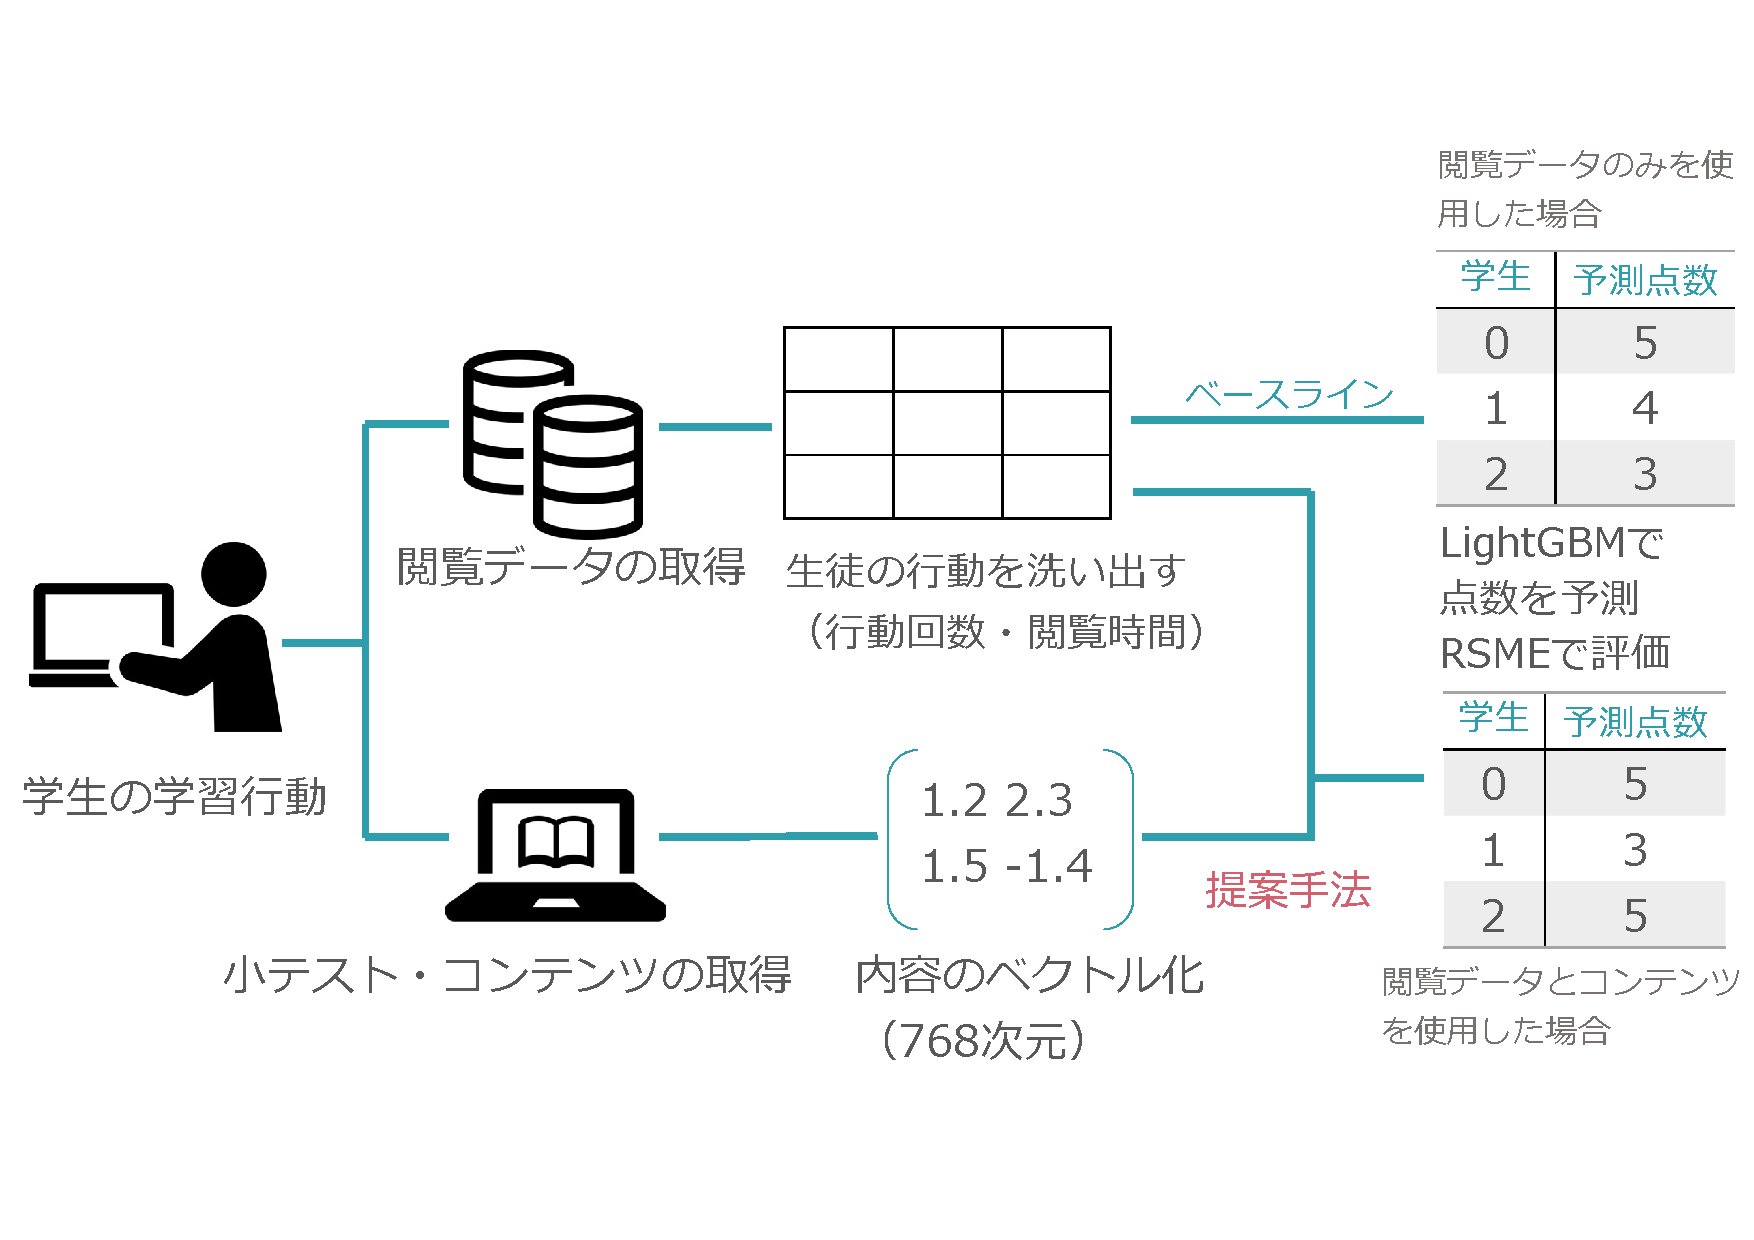
\includegraphics[scale = 0.23]{zentaizo.pdf}
  \vspace{-5mm}
  \caption{本研究の全体像}
  \label{fig:本研究の全体像}
\end{figure}

% 行動特徴量として行動回数洗い出す操作は,すべての操作ではなく,OPEN, NEXT, PREV, CLOSE, PAGE\_JUMP, GETIT, OPEN\_RECOMMENDATION, CLOSE\_RECOMMENDATION, NOTGETIT, ADD MARKER, DELETE MARKER, CLICK\_RECOMMENDATION, open\_timeに絞る.


コンテンツ${c}$に含まれる文章のベクトル化を行い,そのベクトルを行動特徴量に付け加えて点数予測を行う方法である.現在はベクトル化に事前学習済みのSentence-BERT~\cite{sentence-BERT2019}を使用してページ${p^{(c)}}$ごとに768次元のベクトル化を行っている.しかし,ページ内容をベクトル化したものを付け加えただけでは全ての学生が同じベクトルをもつことになるため,ページベクトルに重みづけを行うことで学生ごとに違ったベクトルを作成する.重みには各スライドの閲覧時間$t^{(i)}_{(c,p)}$を使用し,学生の閲覧時間が長いスライドほど重要度$w^{(i)}_{(c,p)}$を高く設定する.単純に閲覧時間が長いほど重要度を高くすると異常に長い時間閲覧していると記録されている可能性があるため,一度に同じページを見ている時間が17分(1020秒)以上の場合はセッションタイムアウトによりCLOSEが記録されなかった,もしくは長時間放置されているものとしてフィルタ―をかける.フィルタ―をかけたあとの閲覧時間をページごとに足し合わせた時間を使用し,重要度を求める.各講義回ごとに閲覧時間が一番長いページを$t^{(c)}_{max}$とし,そこから連続的に重要度を求める.
% 重要度は以下のように求める.
\begin{align}
  w^{(i)}_{(c,p)} = \frac{t^{(i)}_{(c,p)}}{t^{(c)}_{max}}
\end{align}
ベクトルは各スライドに対し作成されているため,このままでは行動特徴量が大きくなるので,重みづけを行ったベクトルを足し合わせることでベクトルの圧縮を行う.

% 学生番号を$i$とし,各学生の閲覧時間
% c=[1,1+,2-1,2-2,3,4,5,6,7]
% p=[週によって違う]
% 閲覧時間はさらっと言って大丈夫なんか?ページ移動からだすってかく?必要ある?

% 使用する行動は記録されている全ての行動ではなく,絞っている.(ベクトル圧縮のため)言わないといけない(下でかく?)
% 使っている行動の選定理由は行動だけで週ごと予測をしたときに重要であるとでてきた行動(正確には削ったのが、どの週でも重要度が0ってでてきた行動)

% 講義時間外も含む全てのデータと講義時間内\&前後1時間に絞ったのは自分のやりたいこと、目的的に講義時間内に絞ることは必要なのではと思ったから





\section{評価}
\label{sec:evaluation}

\subsection{使用データセット}

2020年に九州大学で行われた講義で使用されたBookRollシステムから得た閲覧データとコンテンツ情報,毎週講義後に行われる小テストから得たデータを使用する.講義は80分講義,10分小テストという形式で100名の学生に対し7週間にわたって行われ,閲覧データは合計200,818ログ記録されている.
小テストは5問の択一式の問題で構成され,小テストデータは学生が小テストを提出したタイミングで記録される.小テストデータには問題の文章,学生の選択した選択肢,正解かどうか,提出時間が含まれている.



\subsection{予測・評価方法}

点数予測は小テストごとにLightGBMを使用して行う.5-foldのクロスバリデーションでRSMEを計算し,評価する.
評価には小テストデータから得た,小テストごとに求めた5点満点の点数を使用する.
2週目は2つのコンテンツが使用され,小テストが2回分行われているため,2週目(1),2週目(2)と分けて点数予測を行っている.
今回は行動特徴量を講義時間外の行動もすべて含む行動特徴量を使用して点数予測を行った結果と,講義時間内と前後1時間の行動に絞った行動特徴量を使用して点数予測を行った結果をそれぞれ評価し,ベースラインの結果と提案手法の結果を比較する.
行動特徴量として行動回数洗い出す操作はすべての操作ではなく,閲覧時間を除く,行動回数のみを使用し週ごとの点数予測をLightGBMで行った結果,どの週でもImportanceが0であった行動を除いたOPEN, NEXT, PREV, CLOSE, PAGE\_JUMP, GETIT, OPEN\_RECOMMENDATION, CLOSE\_RECOMMENDATION, NOTGETIT, ADD MARKER, DELETE MARKER, CLICK\_RECOMMENDATION, open\_timeに絞る.
次元数はコンテンツごとに異なり,1週目1,042次元,2週目(1)1,627次元,2週目(2)1,575次元,3週目1,159次元,4週目1,406次元,5週目1,146次元,6週目1,367次元,7週目1,835次元である.

% 次元数どうやってかく?表?言葉?表にするとまた伸びる


% Importanceが0であったかどうかはわからないけど先生たちに必要ないって言われた行動も消しています.
% 使用operation
% ['OPEN', 'NEXT', 'PREV', 'CLOSE', 'PAGE_JUMP', 'GETIT', 'OPEN_RECOMMENDATION', 'CLOSE_RECOMMENDATION', 'NOTGETIT', 'ADD MARKER', 'DELETE MARKER', 'CLICK_RECOMMENDATION', 'open_time']

% 削るoperation
% ['TIMER_STOP', 'TIMER_PAUSE', 'MEMO_TEXT_CHANGE_HISTORY']
% 理由:TIMERに関しては無視していいって言われた
% MEMO~の方は学生がメモしている最中が全部記録されるので打ち間違いとかも入る(いらない)

% ['ADD MEMO', 'ADD BOOKMARK', 'LINK_CLICK', 'CHANGE MEMO', 'BOOKMARK_JUMP', 'DELETE BOOKMARK', 'DELETE_MEMO', 'SEARCH', 'SEARCH_JUMP', 'ADD_HW_MEMO']
% 理由:どの週でもLightGBMで重要ってでてこないから

\subsection{結果}

ベースラインの手法と提案手法で小テストごとに点数予測を行い,求めたRMSEの平均を図3に示す.
小テストごとの詳しいRMSEの値は表1に示している.
表1はベースラインと提案手法を比較し,小テストごとに色が濃い方がRMSEの値が小さくなっている.

% 白黒らしいので色薄くした方が良いかも
% 色無くして言葉で説明する?↓
% 2週目-2,3週目,5週目,6週目ではどちらの場合でも提案手法の方がベースラインと比較して小さい値をとっている.とか


\begin{figure}[h]
  \centering
  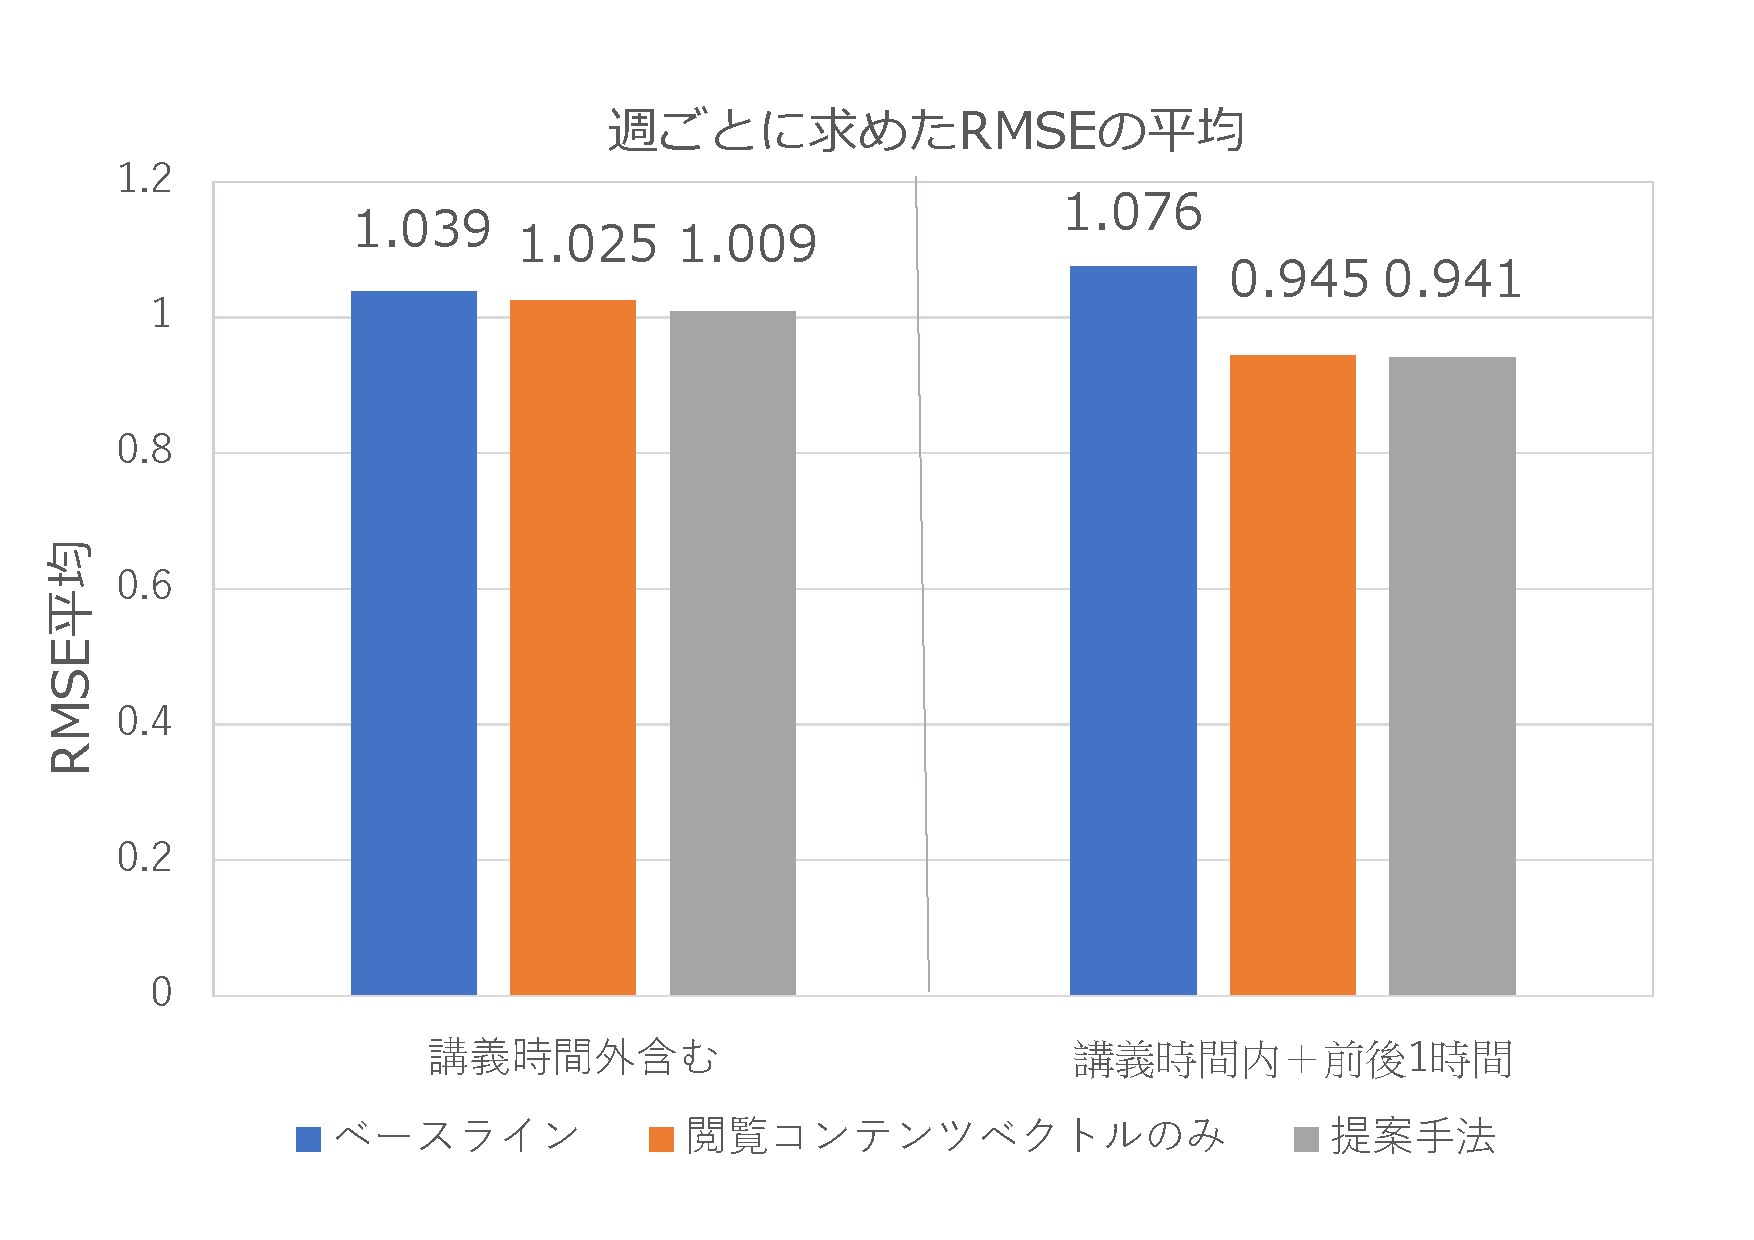
\includegraphics[scale = 0.25]{RMSE.pdf}
  % \vspace{-10mm}
  \caption{小テストごとに求めたRMSEの平均}
  \label{fig:小テストごとに求めたRMSEの平均}
\end{figure}



\begin{table}[h]
  \centering
  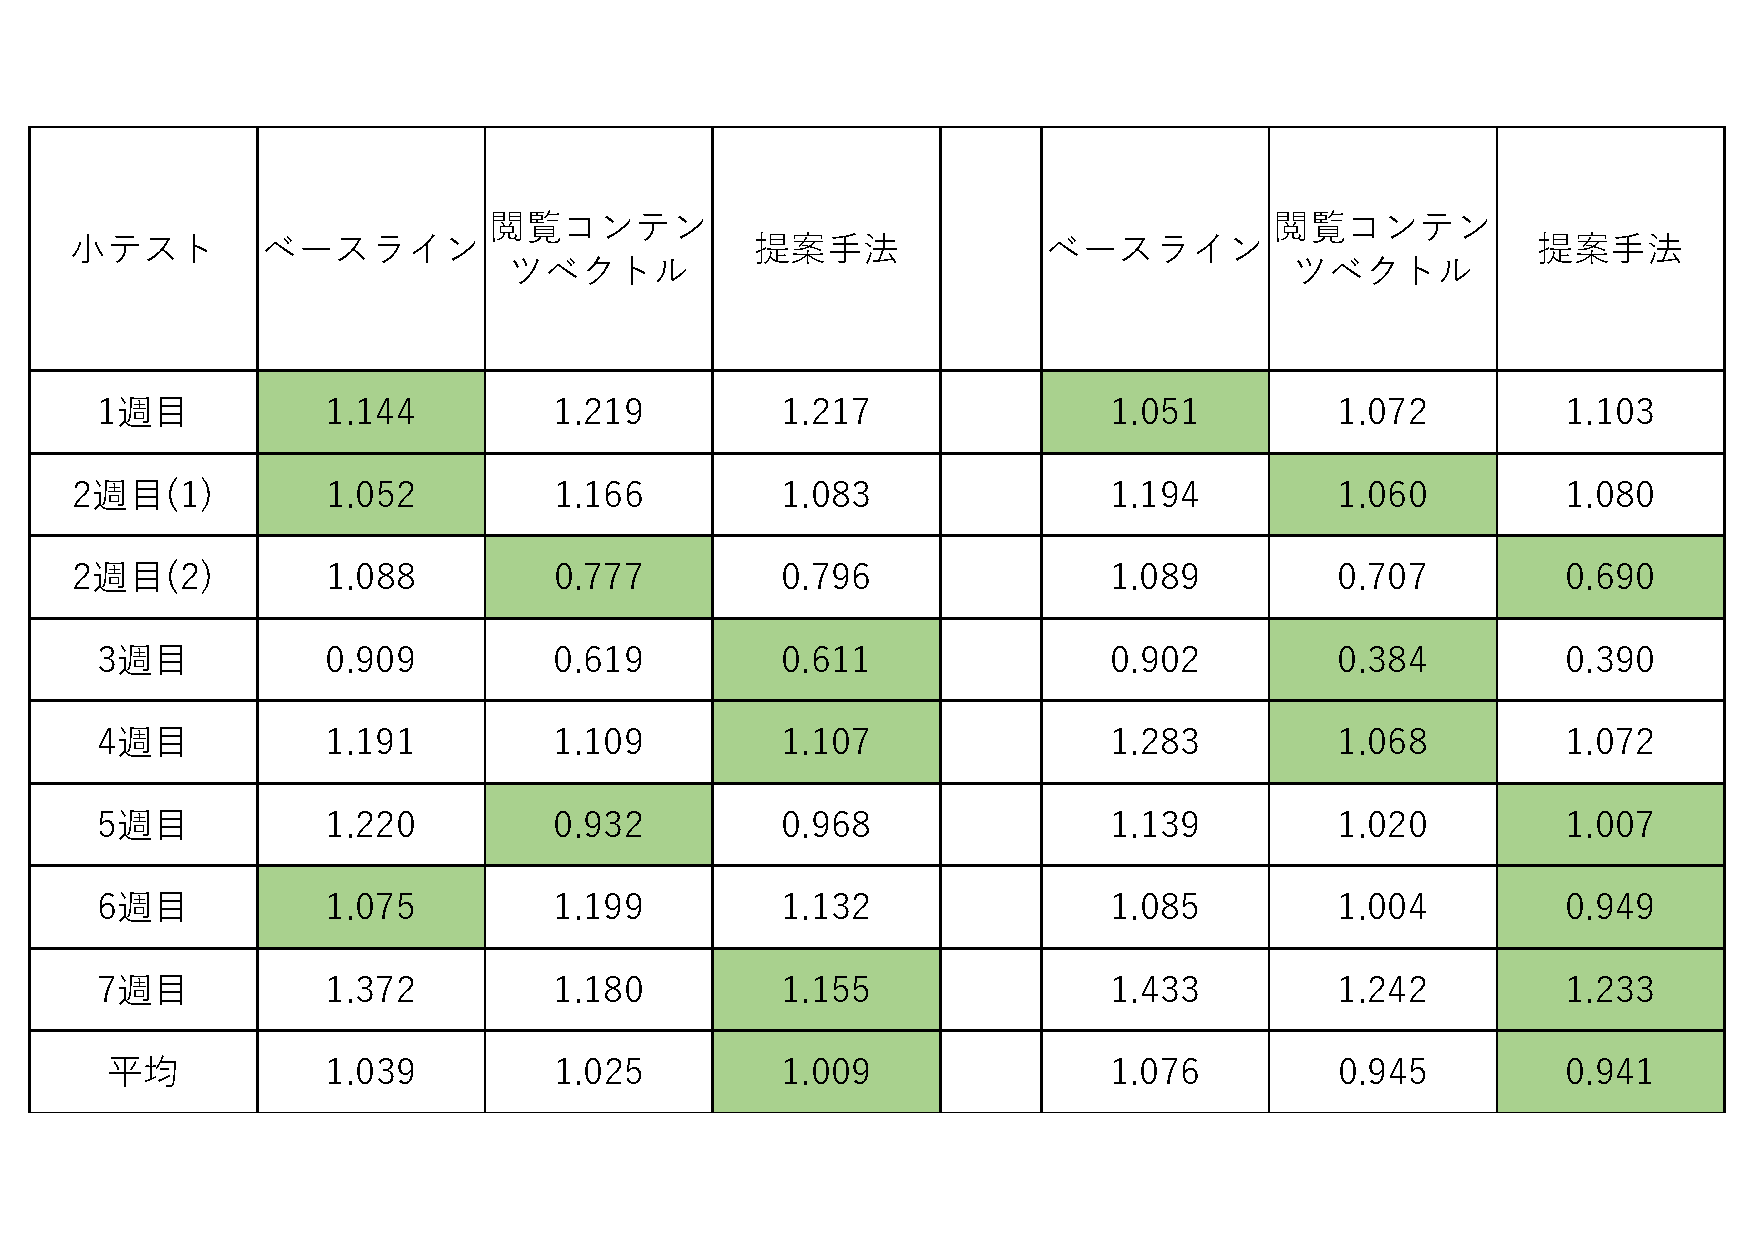
\includegraphics[scale = 0.25]{RMSEhyov3_.pdf}
  % \vspace{-10mm}
  \caption{小テストごとに求めたRMSEの平均\\講義時間外含む(左2列)講義時間内\&前後1時間(右2列)}
  \label{tb:小テストごとのRMSE(表)}
\end{table}


\subsection{課題}
% 課題?考察?まとめ?
結果から,学生の行動を講義時間内(前後1時間含む)に絞ることは点数予測の精度向上に繋がる.また,ベースラインと比べて提案手法ではRMSEの値が下がっていることよりコンテンツ内容を含めることは点数予測の精度向上に繋がり,学習行動の中ではスライドの閲覧時間がより重要であると言える.
本研究では実験していないが,行動の重要度に加え,スライドの重要度を変えることでより高い精度を期待できるのではないだろうか.
% もう少し書きます



\vspace{2mm}
\noindent{\bf 謝辞} \quad
本研究の一部は科研費JP19H04226の補助を受けて行った.

% https://www.jsps.go.jp/j-grantsinaid/16_rule/rule.html#shaji


{
\footnotesize
% \bibliographystyle{jplain}  % LastNameのアルファベット順
\bibliographystyle{junsrt}  % 引用順
\bibliography{ipsjkogishi}  % sample.bib の場合(bibファイル名に合わせて変更すること)
%% bibtex を使わない場合は上の2行をコメントアウトして以下に列挙

% ちょっと微妙journalとかになにかけばいいかにわからないです.
% 論文あった場所bibにおいてます.


% \begin{thebibliography}{10}
% \bibitem{Rodrigue:IUI2015}
% M. Rodrigue, J. Son, B. Giesbrecht, M. Turk, T. H\"{o}llerer.
% \newblock Spatio-Temporal Detection of Divided Attention in Reading Applications Using EEG and Eye Tracking.
%   \newblock In {\em IUI}, pages 121--125. 2015.
% \end{thebibliography}
}


\end{document}
